\documentclass[a4paper,10pt]{article}

\usepackage{cite}
\usepackage{graphicx}
\usepackage{fancyhdr}
\usepackage{amstext,amsmath,amssymb}
\usepackage[shortlabels]{enumitem}

\setlength{\oddsidemargin}{0cm} %
\setlength{\evensidemargin}{0cm} %
\setlength{\topmargin}{0cm} %
\setlength{\textwidth}{16cm} %
\setlength{\textheight}{22.5cm} %

\pagestyle{empty}
\newcommand{\assunto}{PARAFAC and Tensor Rank}

\sloppy

\begin{document}

\thispagestyle{empty}

\begin{center}
  
    
\includegraphics[scale=0.10]{figs/icon.png}
    
    \LARGE{Universidade Federal do Ceará}
    
    \LARGE{Centro de Tecnologia}
    
    \LARGE{Departamento de Engenharia de Teleinformática}
    
    \LARGE{Engenharia de Teleinformática}
    
    \vspace{180pt}
      
    \LARGE{Multilinear Algebra}
      
    \LARGE{Computational Homeworks}
      
    \vspace{100pt}
    
\end{center}

\vspace{25pt}

\begin{flushleft}
	\begin{tabbing}
		Student \qquad Kenneth Brenner dos Anjos Benício – 519189\\
	   \qquad\qquad\qquad\= \\
		Professor\> Andre Lima Ferrer de Almeida \\
		Course \> Multilinear Algebra - TIP8419\\
	\end{tabbing}
\end{flushleft}

\vspace{25pt}

\begin{center}
    Fortaleza, 2022
\end{center}
\thispagestyle{empty}

\newpage

\thispagestyle{empty}

\newpage
\section*{Homework 0 \\ Kronecker Product Run Time}

    \subsection*{Run Time Perfomance of Sequential Kronecker Products}

    In here I will briefly analyze the run time performance of the inverse operator while also using the Kronecker Product. In the first case the number of products is fixed while the number of columns is varying. 
    In the second case we have a varying number of products for a fixed number of columns. In both cases is possible to see that is preferable to first invert the matrices before applying the Kronecker operator.  
    
    \begin{figure}[ht!]
        \centering 
        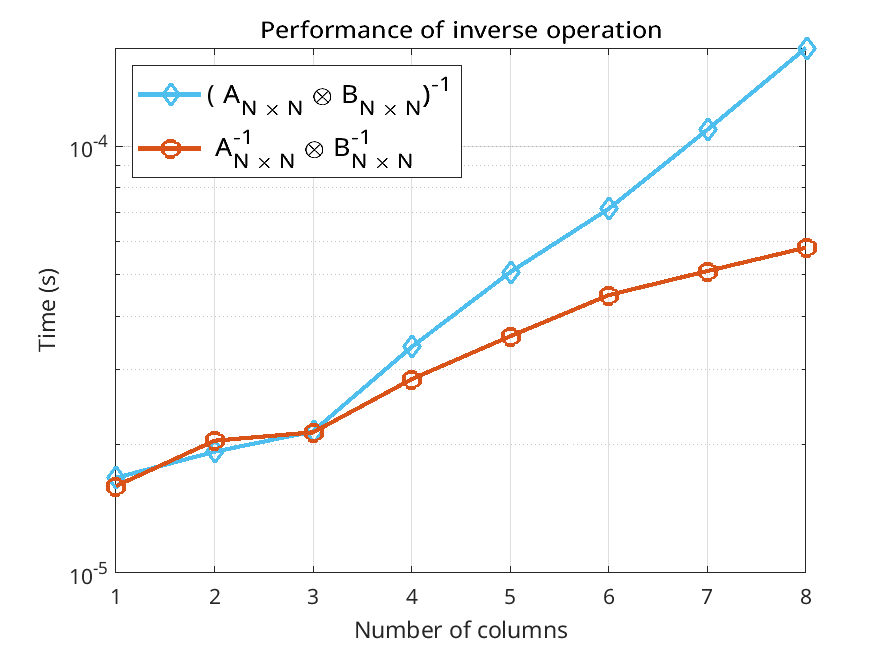
\includegraphics[width=0.75\linewidth]{figs/hw0a1.png} \par 
        \caption{Monter Carlo Experiment with 5000.}
        \label{fig:hw0a1} 
    \end{figure}

    \begin{figure}[ht!]
        \centering 
        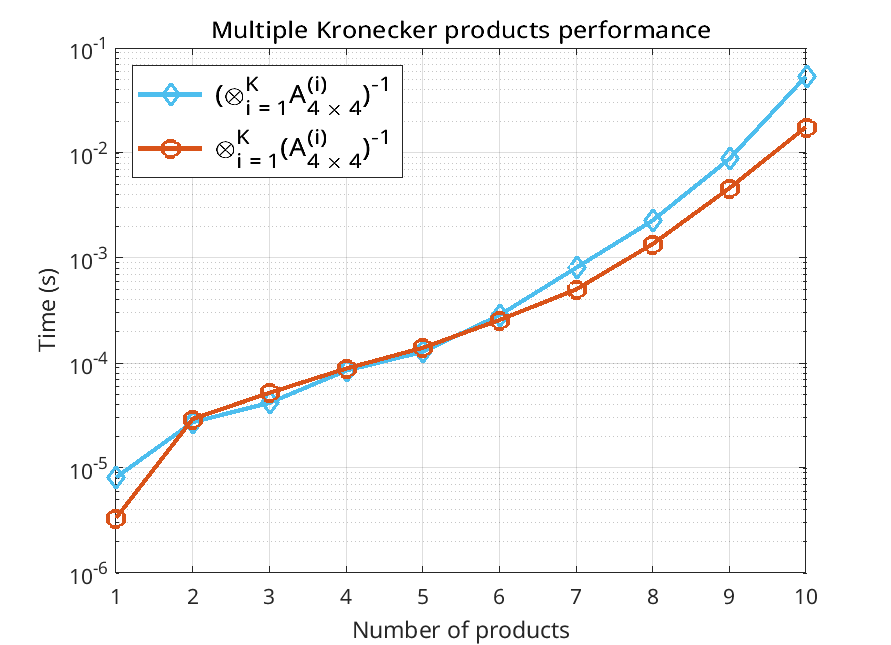
\includegraphics[width=0.75\linewidth]{figs/hw0a2.png} \par 
        \caption{Monter Carlo Experiment with 10000 runs.}
        \label{fig:hw0a2} 
    \end{figure}

    \subsection*{Show that $\text{eig}(\boldsymbol{A} \otimes \boldsymbol{B}) = \text{eig}(\boldsymbol{A}) \otimes \text{eig}(\boldsymbol{B})$}

    By using the eigenvalue decomposition (eig) of two matrices and apply the Kronecker Product to them it is possible to reach the intended result

    \begin{align}
        \boldsymbol{A} \otimes \boldsymbol{B} &= (\boldsymbol{C}_{1} \boldsymbol{\Lambda_{1}} \boldsymbol{C}^{-1}_{1}) \otimes (\boldsymbol{C}_{2} \boldsymbol{\Lambda_{2}} \boldsymbol{C}^{-1}_{2}), \\
        \boldsymbol{A} \otimes \boldsymbol{B} &= (\boldsymbol{C}_{1} \boldsymbol{\Lambda_{1}} \otimes \boldsymbol{C}_{2} \boldsymbol{\Lambda_{2}}) (\boldsymbol{C}^{-1}_{2} \otimes \boldsymbol{C}^{-1}_{2}), \\
        \boldsymbol{A} \otimes \boldsymbol{B} &= (\boldsymbol{C}_{1} \otimes \boldsymbol{C}_{2}) (\boldsymbol{\Lambda_{1}} \otimes \boldsymbol{\Lambda_{2}}) (\boldsymbol{C}^{-1}_{2} \otimes \boldsymbol{C}^{-1}_{2}), \\
        \text{eig}(\boldsymbol{A} \otimes \boldsymbol{B}) &= (\boldsymbol{\Lambda_{1}} \otimes \boldsymbol{\Lambda_{2}}) = \text{eig}(\boldsymbol{A}) \otimes \text{eig}(\boldsymbol{B}) 
    \end{align}

\newpage
\section*{Homework 1 \\ Hadamard, Kronecker and Khatri-Rao Products}

    \subsection*{Run Time Perfomance of Hadamard Product}

    \begin{figure}[ht!]
        \centering 
        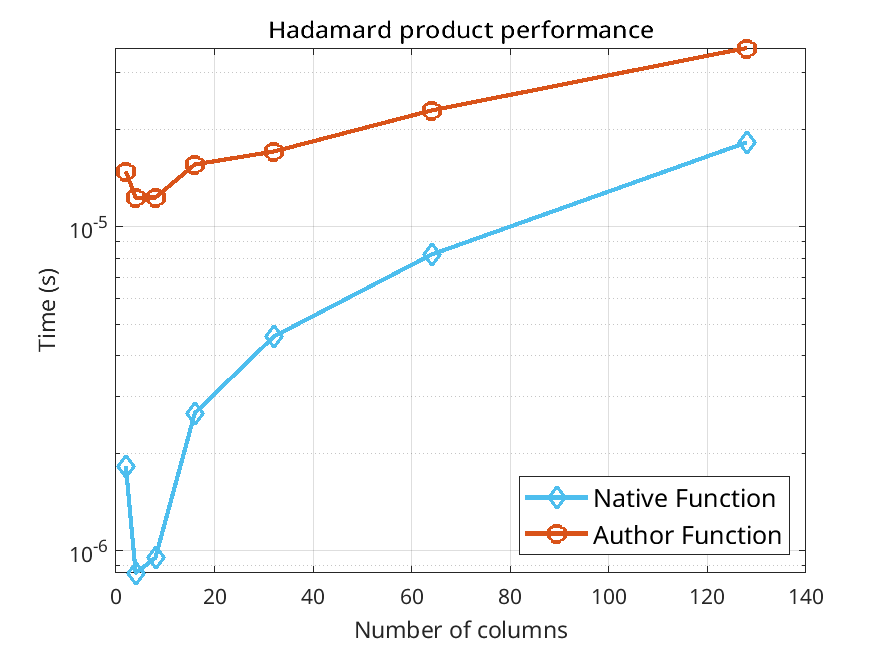
\includegraphics[width=0.75\linewidth]{figs/hw1a1.png} \par 
        \caption{Monter Carlo Experiment with 1000 runs.}
        \label{fig:hw1a1} 
    \end{figure}

    \subsection*{Run Time Perfomance of Kronecker Product}

    \begin{figure}[ht!]
        \centering 
        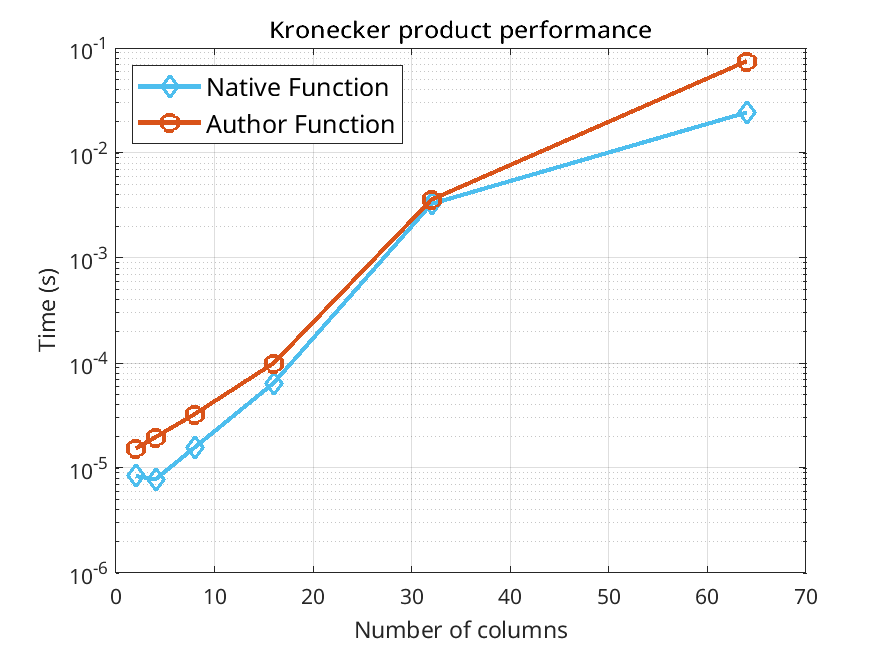
\includegraphics[width=0.75\linewidth]{figs/hw1a2.png} \par 
        \caption{Monter Carlo Experiment with 1000 runs.}
        \label{fig:hw1a2} 
    \end{figure}

    \subsection*{Run Time Perfomance of Khatri-Rao Product}

    \begin{figure}[ht!]
        \centering 
        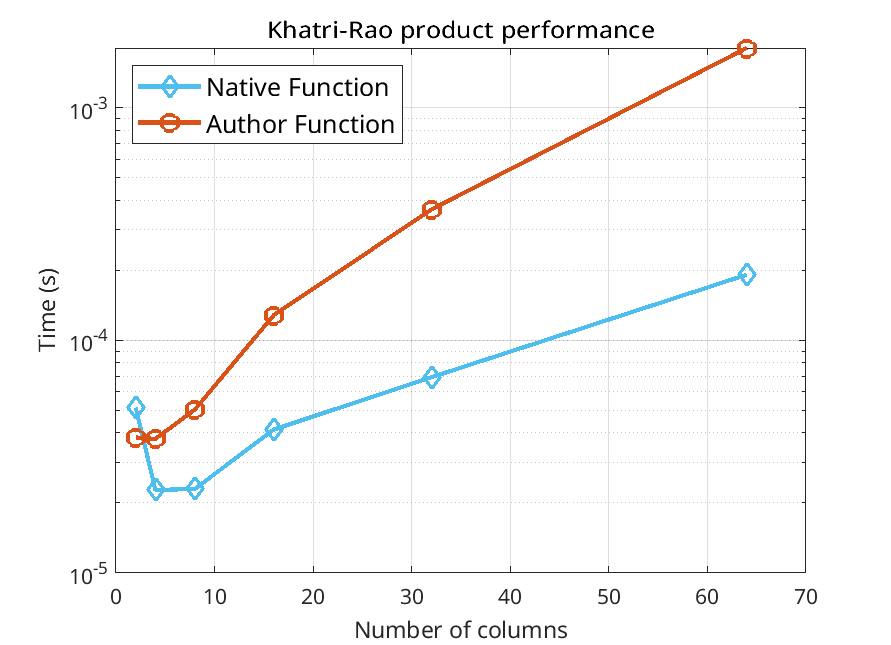
\includegraphics[width=0.75\linewidth]{figs/hw1a3.png} \par 
        \caption{Monter Carlo Experiment with 1000 runs.}
        \label{fig:hw1a3} 
    \end{figure}

\newpage
\section*{Homework 2 \\ Khatri-Rao Product Run Time}

    \subsection*{Run Time Performance of Khatri-Rao Product for Different Implementations}

    In Figures \ref{fig:hw2a1} and \ref{fig:hw2a2} we can see the processing time for the considered methods to compute the pseudoinverse of a Khatri-Rao product for the cases
    where we have two and four columns in each matrix. To draw the curves it was implemented a Monte Carlo Experiment with only 250 runs for each value $N$ of rows with $N \in \{2, 4, 8, 16, 32, 64\}$.
    For both cases we can see a clear advantage in using the third method as the dimmensions of the matrices increases. In a similar maner, we can also observe that the second method is a bit better than the first however 
    not as good as the third. To see a better behavior for these methods it should be necessary to increase the number of rows to better analyse the advantages of each one, however due to technical constraints 
    I could not increase as much as I wanted. 

    \begin{align}
        (\boldsymbol{A} \diamond \boldsymbol{B})^{\dagger} &= \text{pinv}(\boldsymbol{A} \diamond \boldsymbol{B}), \\
        (\boldsymbol{A} \diamond \boldsymbol{B})^{\dagger} &= [(\boldsymbol{A} \diamond \boldsymbol{B})^{\text{T}} (\boldsymbol{A} \diamond \boldsymbol{B})]^{-1} (\boldsymbol{A} \diamond \boldsymbol{B})^{\text{T}}, \\
        (\boldsymbol{A} \diamond \boldsymbol{B})^{\dagger} &= [(\boldsymbol{A}^{\text{T}}\boldsymbol{A})(\boldsymbol{B}^{\text{T}}\boldsymbol{B})]^{-1} (\boldsymbol{A} \diamond \boldsymbol{B})^{\text{T}}, 
    \end{align}

    \begin{figure}[ht!]
        \centering 
        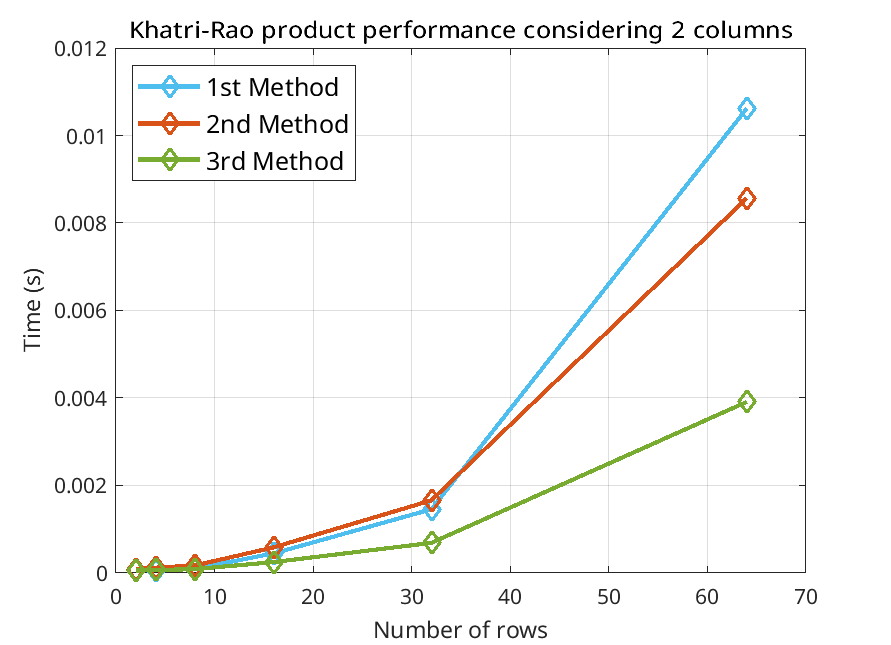
\includegraphics[width=0.75\linewidth]{figs/hw2a1.png} \par 
        \caption{Monter Carlo Experiment with 250 runs and R = 2.}
        \label{fig:hw2a1} 
    \end{figure}

    \begin{figure}[ht!]
        \centering 
        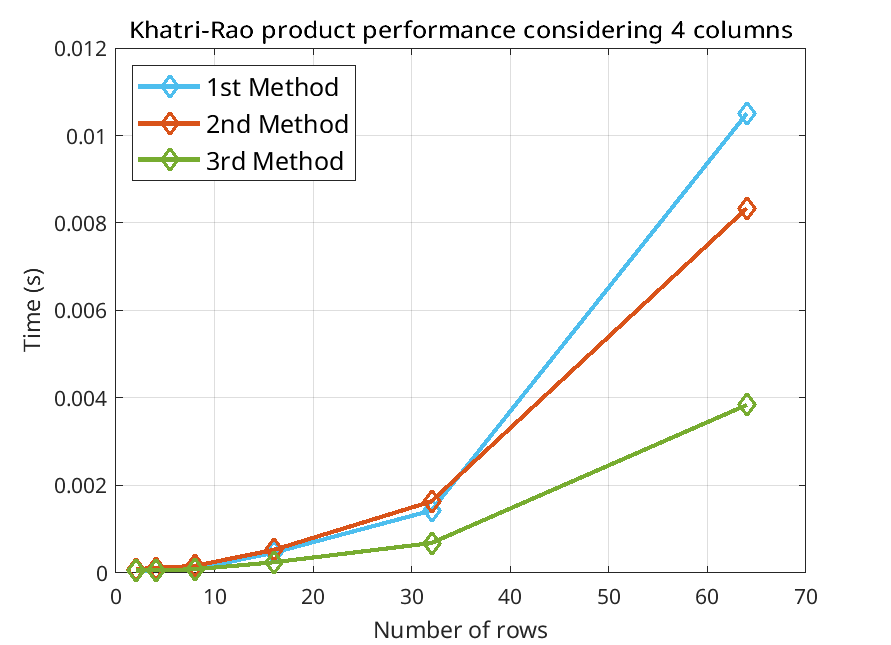
\includegraphics[width=0.75\linewidth]{figs/hw2a2.png} \par 
        \caption{Monter Carlo Experiment with 250 runs and R = 4.}
        \label{fig:hw2a2} 
    \end{figure}

    \subsection*{Run Time Perfomance of Sequential Khatri-Rao Products}

    \begin{figure}[ht!]
        \centering 
        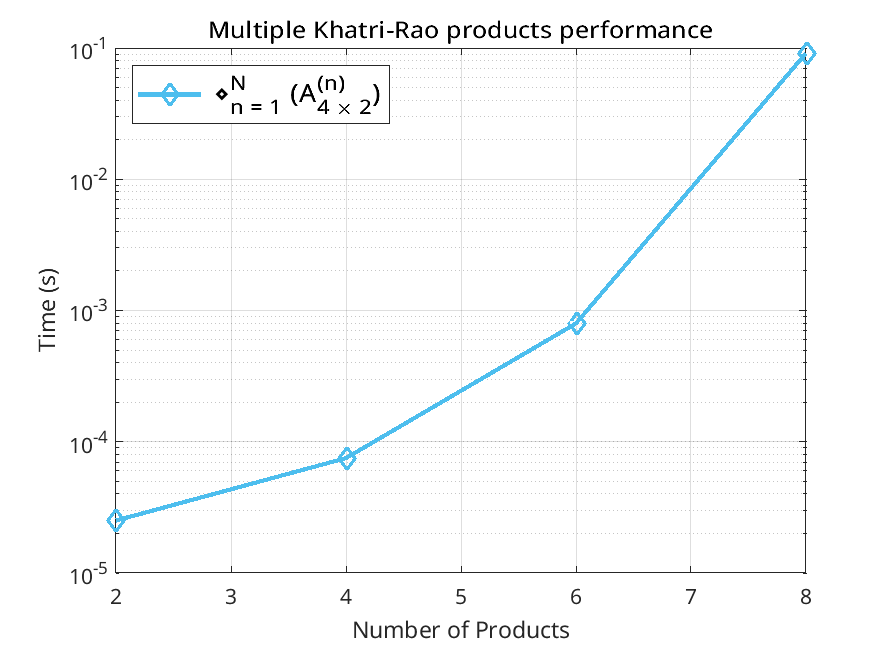
\includegraphics[width=0.75\linewidth]{figs/hw2a3.png} \par 
        \caption{Monter Carlo Experiment with 250 runs.}
        \label{fig:hw2a3} 
    \end{figure}

\newpage
\section*{Homework 3 \\ Least-Squares Khatri-Rao Factorization (LSKRF)}

    \subsection*{Implementation LSKRF}

    \begin{align}
        \left(\hat{\boldsymbol{A}}, \hat{\boldsymbol{B}}\right) = \underset{\boldsymbol{A}, \boldsymbol{B}}{\text{min}} \left|\left| \boldsymbol{X} - \boldsymbol{A} \diamond \boldsymbol{B} \right|\right|^2_{\text{F}},
    \end{align}

    \begin{table}[ht!]
        \centering
        \begin{tabular}{|l|l|l|l|}
        \hline
        NMSE($\boldsymbol{X}, \boldsymbol{\hat{X}}$) & NMSE($\boldsymbol{A}, \boldsymbol{\hat{A}}$) & NMSE($\boldsymbol{B}, \boldsymbol{\hat{B}}$) \\ \hline
        -623.4093 & +11.5658 & +7.8479 \\ \hline
        \end{tabular}
    \end{table}

    \subsection*{Monte Carlo Experiment}

    \begin{figure}[ht!]
        \centering 
        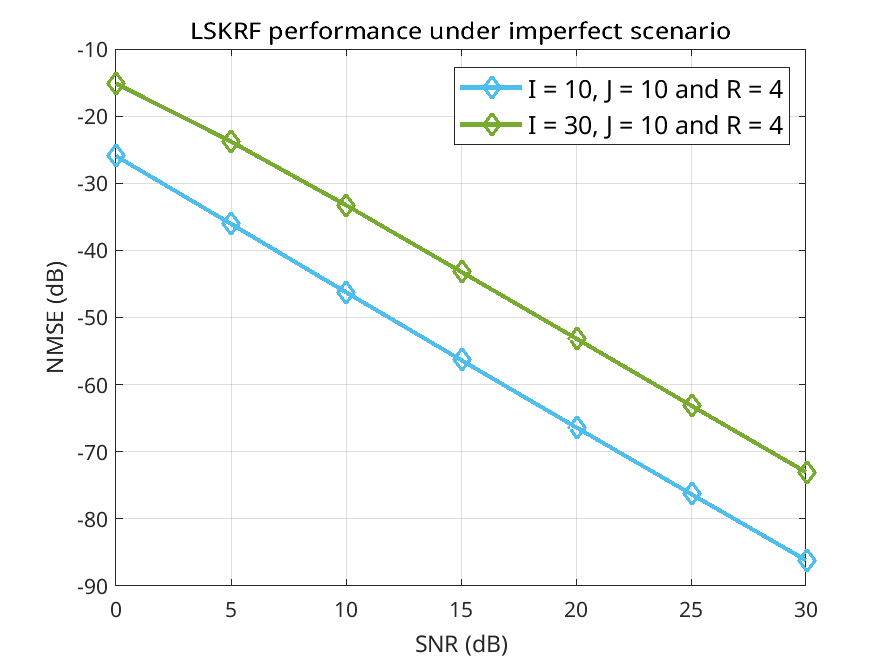
\includegraphics[width=0.75\linewidth]{figs/hw3.png} \par 
        \caption{Monter Carlo Experiment with 1000 runs for LSKRF algorithm.}
        \label{fig:hw3} 
    \end{figure}

\newpage
\section*{Homework 4 \\ Least Squares Kronecker Product Factorization (LSKronF)}

    \subsection*{Implementation LSKronF}

    \begin{align}
        \left(\hat{\boldsymbol{A}}, \hat{\boldsymbol{B}}\right) = \underset{\boldsymbol{A}, \boldsymbol{B}}{\text{min}} \left|\left| \boldsymbol{X} - \boldsymbol{A} \otimes \boldsymbol{B} \right|\right|^2_{\text{F}},
    \end{align}

    \begin{table}[ht!]
        \centering
        \begin{tabular}{|l|l|l|l|}
        \hline
        NMSE($\boldsymbol{X}, \boldsymbol{\hat{X}}$) & NMSE($\boldsymbol{A}, \boldsymbol{\hat{A}}$) & NMSE($\boldsymbol{B}, \boldsymbol{\hat{B}}$) \\ \hline
        -619.2196 & +13.5472 & +9.5922 \\ \hline
        \end{tabular}
    \end{table}

    \subsection*{Monte Carlo Experiment}

    \begin{figure}[ht!]
        \centering 
        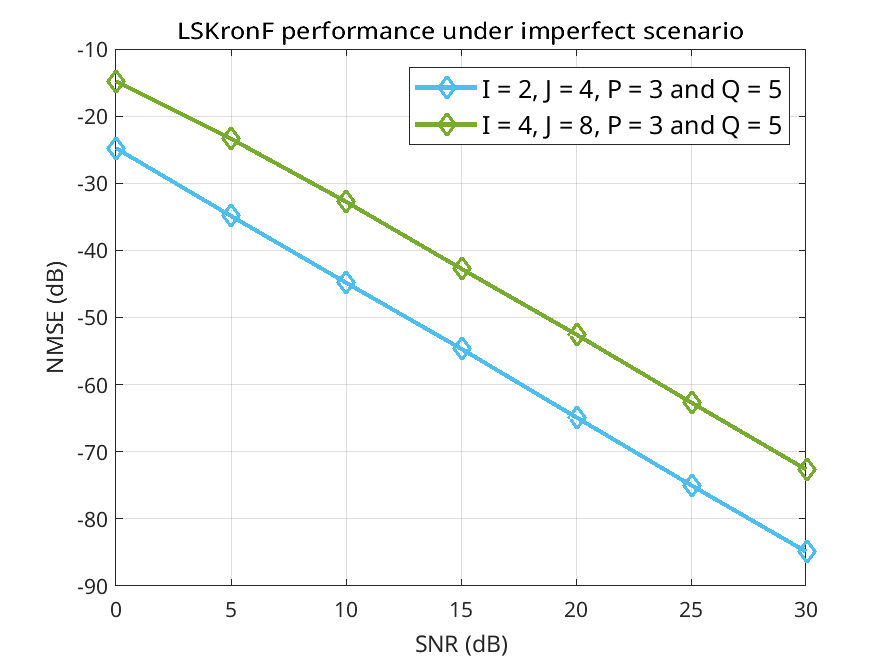
\includegraphics[width=0.75\linewidth]{figs/hw4.png} \par 
        \caption{Monter Carlo Experiment with 1000 runs for LSKronf algorithm.}
        \label{fig:hw4} 
    \end{figure}

\newpage
\section*{Homework 5 \\ Kronecker Product Singular Value Decomposition (KPSVD)}

    \subsection*{Implementation KPSVD}

    \begin{align}
        \boldsymbol{X} = \sum^{r_{kp}}_{k = 1} \sigma_{k} \boldsymbol{U}_{k} \otimes \boldsymbol{V}_{k},
    \end{align}

    In the example is considered that the original matrix has a full rank equals to 9, then two approximations using the KPSVD are provided: One using the full-rank approximation and other using a r-rank approximation $(r < 9)$. 
    The NMSE between some approximations and its original matrix are provided in the sequence

    \begin{table}[ht!]
        \centering
        \begin{tabular}{|l|l|l|l|l|}
        \hline
        Full Rank & Rank = $7$ & Rank = $5$ & Rank = $3$ & Rank = $1$ \\ \hline
        -604.8023 & -51.3722 & -26.7589 & -16.9054 & -6.3068 \\ \hline
        \end{tabular}
    \end{table}

    \subsection*{Validation of KPSVD}

\newpage
\section*{Homework 6 \\ Unfolding, folding, and n-mode product}

    \subsection*{Implementation unfolding, folding and n-mode product}

    \begin{align}
        [\mathcal{X}]_{n} &= \text{unfold}(\mathcal{X}, [I_{1} \cdots I_{N} ], n) \in \mathbb{C}^{I_{n} \times I_{1} \cdots I_{n-1} I_{n+1} \cdots I_{N}}, \\
        \mathcal{X} &= \text{fold}([\mathcal{X}]_{n}, [I_{1} \cdots I_{N} ], n) \in \mathbb{C}^{I_{1} \times \cdots \times I_{N}}, \\
        \mathcal{Y} &= \mathcal{X} \times_{1} \boldsymbol{U}_{1} \times_{2} \cdots \times_{N} \boldsymbol{U}_{N},
    \end{align}

    \subsection*{Validation of unfolding, folding and n-mode product}

\newpage
\section*{Homework 7 \\ High Order Singular Value Decomposition (HOSVD)}

    \subsection*{Implementation HOSVD}

    \begin{table}[ht!]
        \centering
        \begin{tabular}{|l|l|l|l|l|}
        \hline
        NMSE($\mathcal{X}, \mathcal{\hat{X}}$) & NMSE($\mathcal{S}, \mathcal{\hat{S}}$) & NMSE($\boldsymbol{U}_{1}, \boldsymbol{\hat{U}}_{1}$) & NMSE($\boldsymbol{U}_{2}, \boldsymbol{\hat{U}}_{2}$) & NMSE($\boldsymbol{U}_{3}, \boldsymbol{\hat{U}}_{3}$) \\ \hline
        -611.2162 & +7.7656 & +2.6667 & +2.0000 & +1.6063 \\ \hline
        \end{tabular}
    \end{table}

    \subsection*{Validation of HOSVD}
    
    The multilinear rank advantage is maximized when it comes to process sparce tensors since the dimmensions can be greatly reduced without losing of too much relevant information by analysing the profile of its multiples unfoldings.

    \begin{align}
        \mathcal{X} &\in \mathbb{C}^{8 \times 4 \times 10} \to \hat{\mathcal{X}} \in \mathbb{C}^{R_{1} \times R_{2} \times R_{3}}, \\ 
        \mathcal{X} &\in \mathbb{C}^{5 \times 5 \times 5} \to \hat{\mathcal{Y}} \in \mathbb{C}^{P_{1} \times P_{2} \times P_{3}},
    \end{align}


\newpage
\section*{Homework 8 \\ High Order Order Orthogonal Iteration (HOOI)}

    \subsection*{Implementation HOOI}

    \begin{table}[ht!]
        \centering
        \begin{tabular}{|l|l|l|l|l|}
        \hline
        NMSE($\mathcal{X}, \mathcal{\hat{X}}$) & NMSE($\mathcal{S}, \mathcal{\hat{S}}$) & NMSE($\boldsymbol{U}_{1}, \boldsymbol{\hat{U}}_{1}$) & NMSE($\boldsymbol{U}_{2}, \boldsymbol{\hat{U}}_{2}$) & NMSE($\boldsymbol{U}_{3}, \boldsymbol{\hat{U}}_{3}$) \\ \hline
        -607.9515 & +7.2483 & +2.6667 & +3.9622 & +1.16160 \\ \hline
        \end{tabular}
    \end{table}

    \subsection*{Validation of HOOI}

    The multilinear rank advantage is maximized when it comes to process sparce tensors since the dimmensions can be greatly reduced without losing of too much relevant information by analysing the profile of its multiples unfoldings.

    \begin{align}
        \mathcal{X} &\in \mathbb{C}^{8 \times 4 \times 10} \to \hat{\mathcal{X}} \in \mathbb{C}^{R_{1} \times R_{2} \times R_{3}}, \\ 
        \mathcal{X} &\in \mathbb{C}^{5 \times 5 \times 5} \to \hat{\mathcal{Y}} \in \mathbb{C}^{P_{1} \times P_{2} \times P_{3}},
    \end{align}

\newpage
\section*{Homework 9 \\ Multidimensional Least-Squares Khatri-Rao Factorization
(MLS-KRF)}

    \subsection*{Implementation MLS-KRF}

    \begin{align}
        \left(\hat{\boldsymbol{A}}^{(1)}, \cdots, \hat{\boldsymbol{A}}^{(N)}\right) = \underset{\boldsymbol{A}^{(1)}, \cdots, \boldsymbol{A}^{(N)}}{\text{min}} \left|\left| \boldsymbol{X} - \boldsymbol{A}^{(1)} \diamond \cdots \diamond \boldsymbol{A}^{(N)} \right|\right|^2_{\text{F}},
    \end{align}

    \begin{table}[ht!]
        \centering
        \begin{tabular}{|l|l|l|l|}
        \hline
        NMSE($\boldsymbol{X}, \boldsymbol{\hat{X}}$) & NMSE($\boldsymbol{A}_{1}, \boldsymbol{\hat{A}}_{1}$) & NMSE($\boldsymbol{A}_{2}, \boldsymbol{\hat{A}}_{2}$) & NMSE($\boldsymbol{A}_{3}, \boldsymbol{\hat{A}}_{3}$) \\ \hline
        -606.2255 & +3.1432 & +5.0165 & +4.7297 \\ \hline
        \end{tabular}
    \end{table}

    \subsection*{Monte Carlo Experiment}

    \begin{figure}[ht!]
        \centering 
        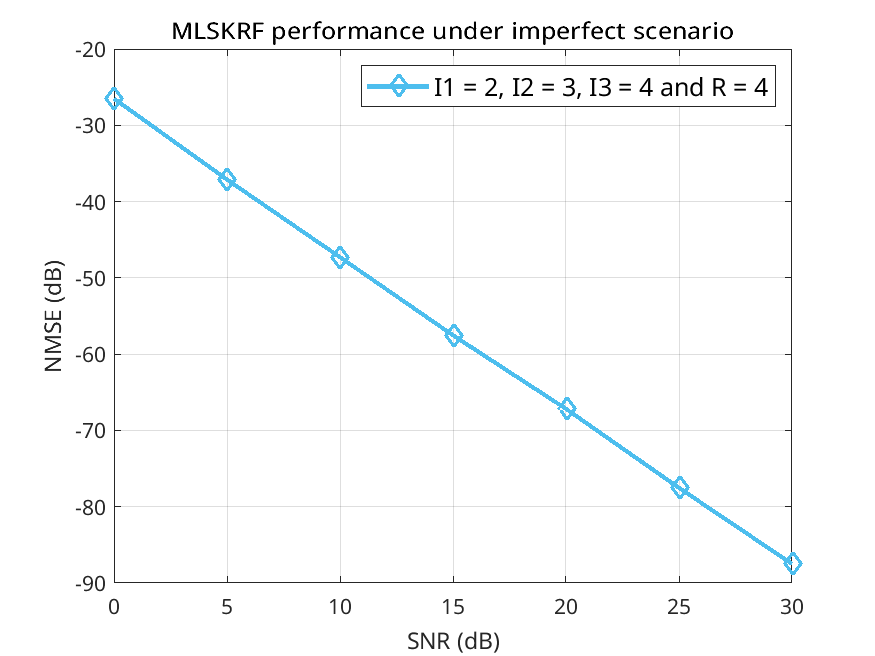
\includegraphics[width=0.75\linewidth]{figs/hw9.png} \par 
        \caption{Monter Carlo Experiment with 1000 runs for MLS-KRF algorithm.}
        \label{fig:hw9} 
    \end{figure}

\newpage
\section*{Homework 10 \\ Multidimensional Least-Squares Kronecker Factorization
(MLS-KronF)}

    \subsection*{Implementation MLS-KronF}

    \begin{align}
        \left(\hat{\boldsymbol{A}}^{(1)}, \cdots, \hat{\boldsymbol{A}}^{(N)}\right) = \underset{\boldsymbol{A}^{(1)}, \cdots, \boldsymbol{A}^{(N)}}{\text{min}} \left|\left| \boldsymbol{X} - \boldsymbol{A}^{(1)} \otimes \cdots \otimes \boldsymbol{A}^{(N)} \right|\right|^2_{\text{F}},
    \end{align}

    \begin{table}[ht!]
        \centering
        \begin{tabular}{|l|l|l|l|}
        \hline
        NNMSE($\boldsymbol{X}, \boldsymbol{\hat{X}}$) & NMSE($\boldsymbol{A}_{1}, \boldsymbol{\hat{A}}_{1}$) & NMSE($\boldsymbol{A}_{2}, \boldsymbol{\hat{A}}_{2}$) & NMSE($\boldsymbol{A}_{3}, \boldsymbol{\hat{A}}_{3}$) \\ \hline
        -605.1941 & +11.9214 & +11.5548 & +6.0950 \\ \hline
        \end{tabular}
    \end{table}

    \subsection*{Monte Carlo Experiment}

    \begin{figure}[ht!]
        \centering 
        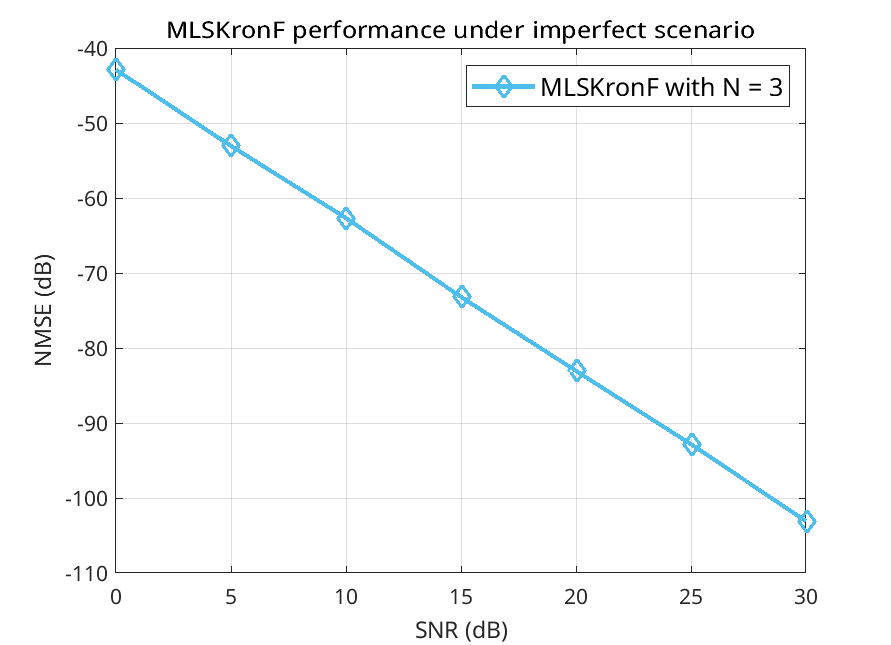
\includegraphics[width=0.75\linewidth]{figs/hw10.png} \par 
        \caption{Monter Carlo Experiment with 1000 runs for MLS-KronF algorithm.}
        \label{fig:hw10} 
    \end{figure}

\newpage
\section*{Homework 11 \\ Alternating Least Squares (ALS) Algorithm}

    \subsection*{Implementation of ALS}

    \begin{align}
        \left(\hat{\boldsymbol{A}}, \hat{\boldsymbol{B}}, \hat{\boldsymbol{C}}\right) = \underset{\boldsymbol{A}, \boldsymbol{B}, \boldsymbol{C}}{\text{min}} \left| \left| \mathcal{X} - \sum^{R}_{r = 1} \boldsymbol{a}_{r} \circ \boldsymbol{b}_{r} \circ \boldsymbol{c}_{r} \right| \right|^{2}_{\text{F}},
    \end{align}

    \subsection*{Monte Carlo Experiment}

    \begin{figure}[ht!]
        \centering 
        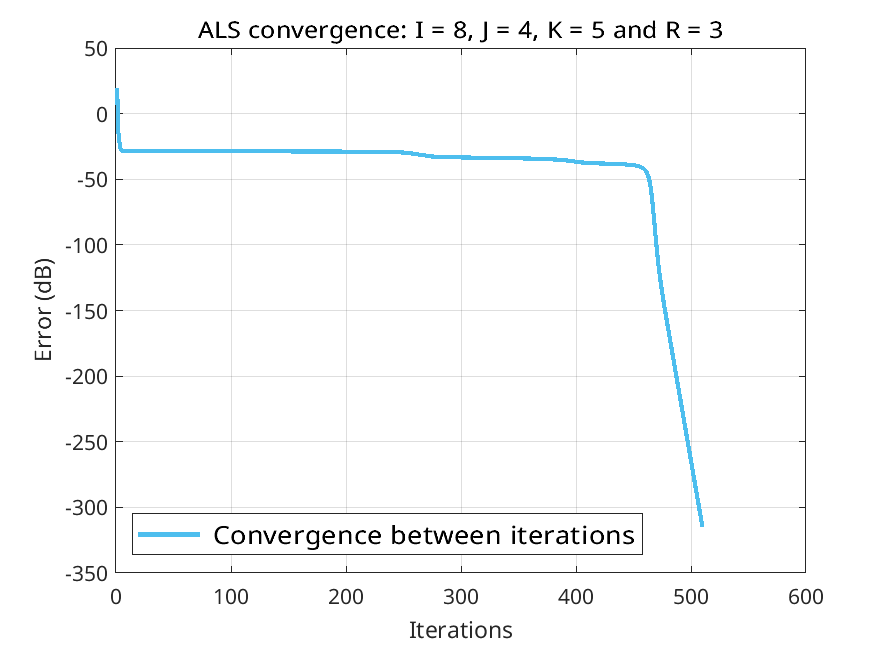
\includegraphics[width=0.75\linewidth]{figs/hw11a1.png} \par 
        \caption{Convergence behavior of ALS algorithm.}
        \label{fig:hw11a1} 
    \end{figure}

    \begin{figure}[ht!]
        \centering 
        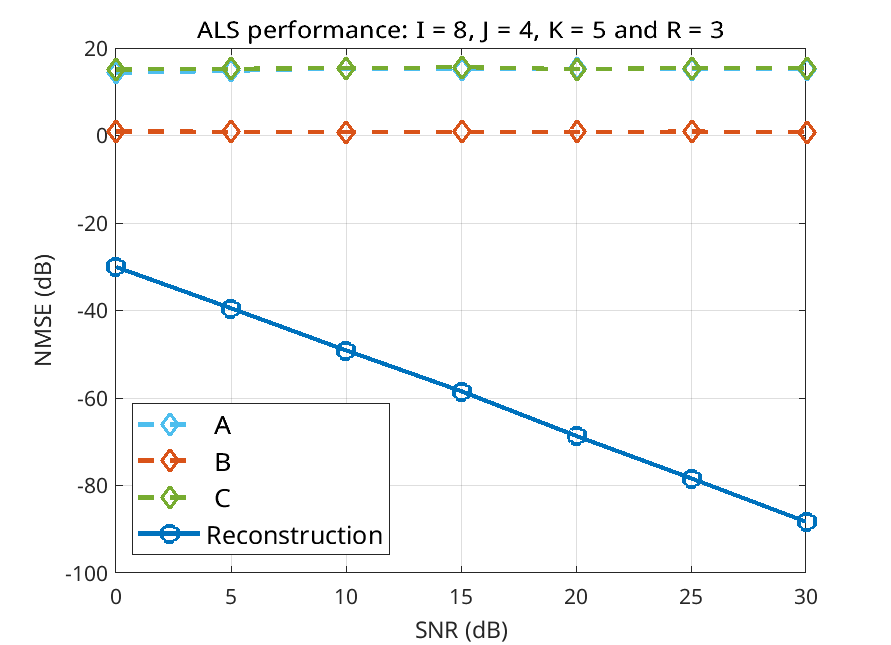
\includegraphics[width=0.75\linewidth]{figs/hw11a2.png} \par 
        \caption{Monter Carlo Experimento with 1000 runs for ALS algorithm.}
        \label{fig:hw11a2} 
    \end{figure}

\newpage
\section*{Homework 12 \\ Tensor Kronecker Product Single Value Decomposition (TKPSVD)}

    \subsection*{Implementation of TKPSVD}

    \begin{align}
        \mathcal{X} = \sum^{R}_{j = 1} \sigma_{i} \mathcal{A}^{(d)}_{j} \otimes \mathcal{A}^{(d - 1)}_{j}  \otimes \cdots \otimes \mathcal{A}^{(1)}_{j},  
    \end{align}

    \begin{table}[ht!]
        \centering
        \begin{tabular}{|l|l|l|l|}
        \hline
        NMSE($\mathcal{X}, \mathcal{\hat{X}}$) & NMSE($\mathcal{A}^{(1)}, \mathcal{\hat{A}}^{(1)}$) & NMSE($\mathcal{A}^{(2)}, \mathcal{\hat{A}}^{(2)}$) & NMSE($\mathcal{A}^{(3)}, \mathcal{\hat{A}}^{(3)}$) \\ \hline
        -625.5192 & +37.0803 & +0.1706 & +32.5731 \\ \hline
        \end{tabular}
    \end{table}

    \subsection*{Monte Carlo Experiment}

    \begin{figure}[ht!]
        \centering 
        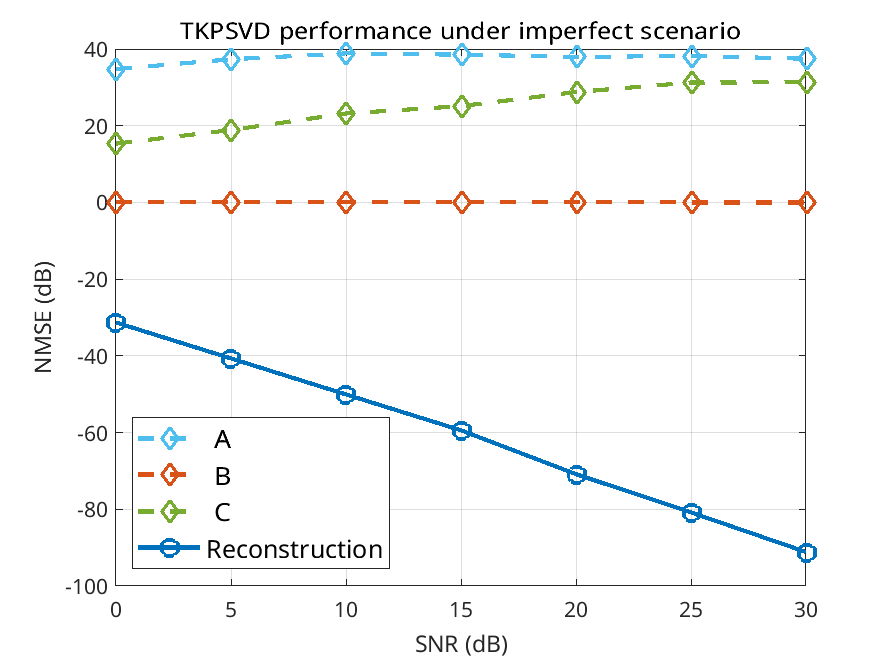
\includegraphics[width=0.75\linewidth]{figs/hw12.png} \par 
        \caption{Monter Carlo Experiment with 1000 runs for TKPSVD algorithm.}
        \label{fig:hw12} 
    \end{figure}

\newpage
\section*{Homework 13 \\ Tensor Train Single Value Decomposition (TTSVD)}

    \subsection*{Implementation of TTSVD}
        
    \begin{align}
        \mathcal{X} = \boldsymbol{G}_{1} \bullet^{1}_{2} \mathcal{G}_{2} \bullet^{1}_{3} \mathcal{G}_{3} \bullet^{1}_{4} \boldsymbol{G}_{4},
    \end{align}

    \begin{align}
        \left(\hat{\boldsymbol{G}_{1}}, \hat{\mathcal{G}_{2}}, \hat{\mathcal{G}_{3}}, \hat{\boldsymbol{G}_{4}}\right) = \underset{\boldsymbol{A}, \boldsymbol{B}, \boldsymbol{C}}{\text{min}} \left| \left| \mathcal{X} - \boldsymbol{G}_{1} \bullet^{1}_{2} \mathcal{G}_{2} \bullet^{1}_{3} \mathcal{G}_{3} \bullet^{1}_{4} \boldsymbol{G}_{4} \right| \right|_{\text{F}},
    \end{align}

    \begin{table}[ht!]
        \centering
        \begin{tabular}{|l|l|}
        \hline
        NMSE($\mathcal{X}, \mathcal{\hat{X}}$) with $R = (3,3,3)$ & NMSE($\mathcal{X}, \mathcal{\hat{X}}$) with $R = (2,2,2)$ \\ \hline 
        -606.0326 & -25.1084 \\ \hline
        \end{tabular}
    \end{table}

    \subsection*{Monte Carlo Experiment}

    \begin{figure}[ht!]
        \centering 
        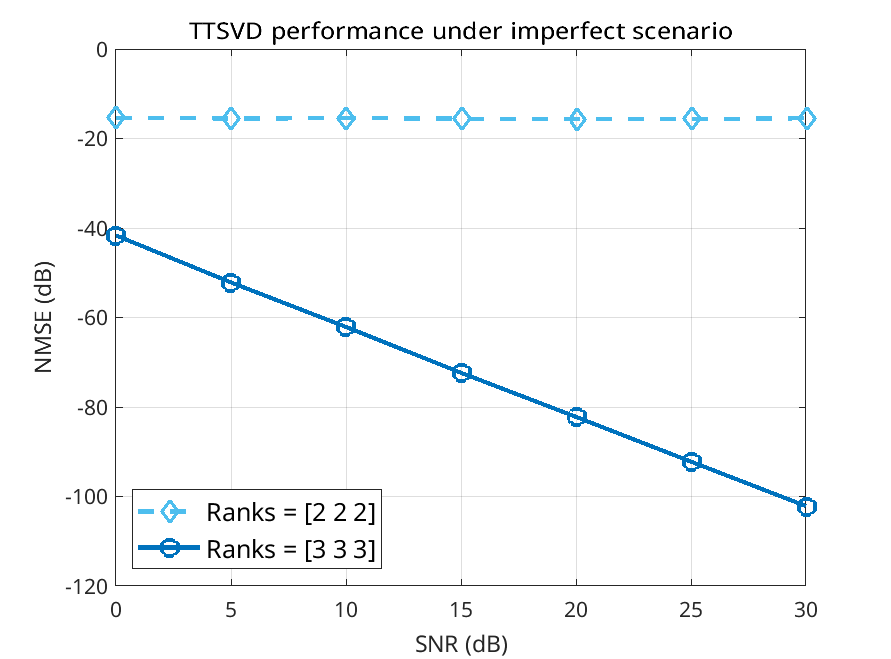
\includegraphics[width=0.75\linewidth]{figs/hw13.png} \par 
        \caption{Monter Carlo Experiment with 1000 runs for TTSVD algorithm.}
        \label{fig:hw13} 
    \end{figure}

%\bibliographystyle{ieeetr}
%\bibliography{bibliography.bib}

\end{document}